\documentclass[prl,twocolumn,amsmath,amssymb,superscriptaddress]{revtex4-2}

\usepackage{graphicx}
\usepackage{verbatim}
\usepackage{braket}
\usepackage{epsfig}
\usepackage{epstopdf}
\usepackage{amsfonts}
\usepackage{amsthm}
\usepackage{amsmath}
\usepackage{amssymb}
\usepackage{color}
\usepackage[dvipsnames,svgnames,table]{xcolor}
\usepackage{hyperref}
\hypersetup{colorlinks=true,linkcolor=NavyBlue,citecolor=BrickRed,urlcolor=NavyBlue}
\usepackage{dsfont}
\usepackage{color}
\usepackage{grffile}
\usepackage{bm}
\usepackage{lipsum}
%end of packages

\begin{document}

\title{PHY180: Pendulum Project}
\author{Luyu Wu Vankerkwijk}
\date{\today}


\maketitle

\section{Introduction}
This paper investigates the non-linear behaviors of a pendulum, largely through experimental analysis, and correlates the findings to an offered linear model of the pendulum:

\begin{equation}
    \theta(t) = A_0e^{-t/\tau}cos\left(\frac{2\pi t}{T}+\phi_0\right)
\end{equation}

This equation (Wilson, 2025) defines the angle of the pendulum as a function of time, where $\theta_0$ and $\phi_0$ are initial conditions, and $\tau$ a constant damping factor.


Experiments were performed using a home-built pendulum, tracked using a high-speed camera. Data was processed to determine experimental relationships between amplitude-period, amplitude-damping, as well as length-period and length-damping were investigated.

\section{Experimental Methods}
The experimental setup consists of a 3 m wool string, wrapped around a cloth hanger attached to a nook in the wall. A cloth hanger is used such that the string can be spooled as to control the length of the pendulum.

The top of the string is bound in such a way that the position of the end of the pendulum does not change. At the bottom of the pendulum, a metal mass with a ring soldered onto it is bound. The mass of the pendulum blob is 54 grams while the full strings is roughly 2 grams. A strand length of $74.5 cm \pm 0.05 cm$ was used in trials where length was kept constant. Note that effective length is affected by the length of boundary and blob.

\begin{figure}[htb]
    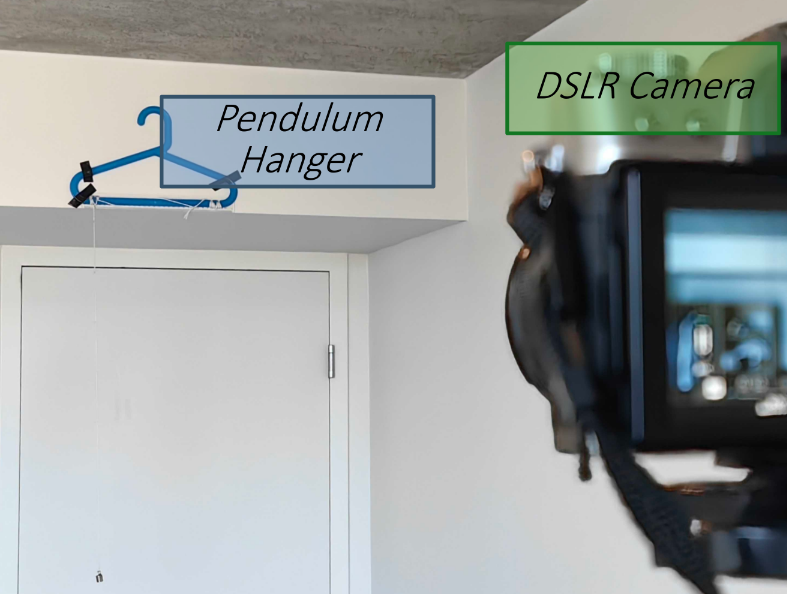
\includegraphics[width=0.68\linewidth]{setup.png}
    \caption{Picture of experimental setup. Pendulum blob is visible in the lower left corner.}
    \label{fig:experiment_setup}
\end{figure}

\newpage

The pendulum system was recorded from approximately 4 meters away (so as to minimize parallax) using a DSLR camera. A shutter speed of $1/1000$ and motion FPS of $60$ were used so as to minimize motion blurring, and maintain a high time resolution.

The pendulum was carefully released by hand, and trials with qualitatively significant out-of-plane movement were rejected (see Appendix B).



\begin{figure}[htb]
    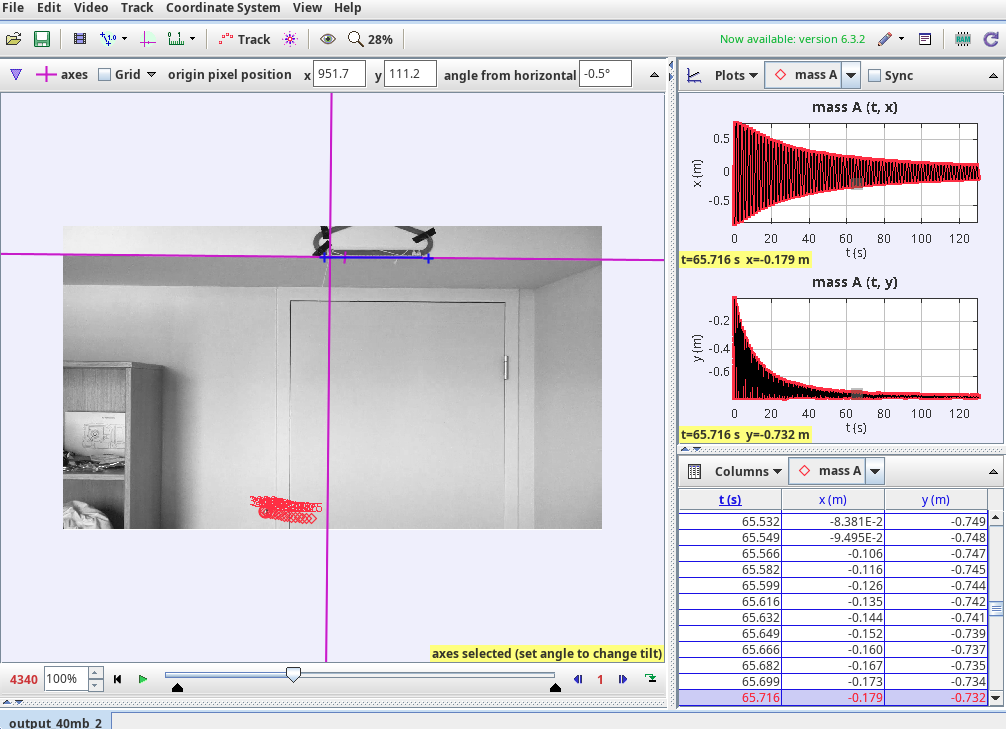
\includegraphics[width=0.7\linewidth]{tracker.png}
    \caption{OSP Tracker software used to obtain projected pendulum position as a function of time.}
    \label{fig:tracker}
\end{figure}

All data was processed in a custom Python script (see Appendix A). In processing the data, we assume that the motion of the pendulum is continuous in reality (for interpolation between points) so as to achieve better time resolution.

SciPy peak detection was performed to find local maximas. Periods were found by iterating through adjascent peak points and finding the time difference ($T_n=t_{n+1}-t_{n}$).

\begin{figure}[htb]
    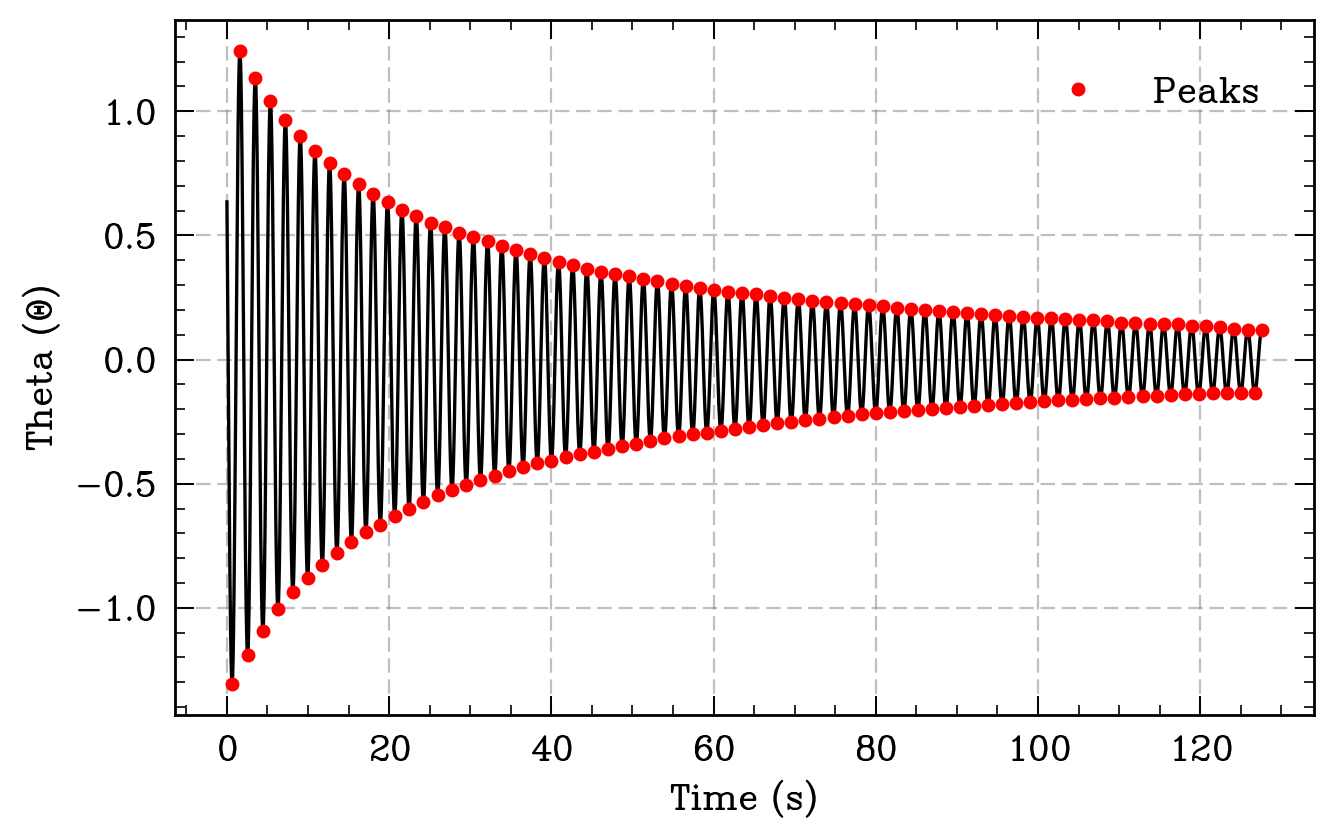
\includegraphics[width=0.8\linewidth]{angle_time.png}
    \label{fig:angle_time}
    \caption{Plot of pendulum angle against time, along with detected peaks.}
\end{figure}

\section{Results}


\subsection{Period Non-Linearity}
\vspace{-20pt}
\begin{figure}[htb]
    \hspace{-20pt}
    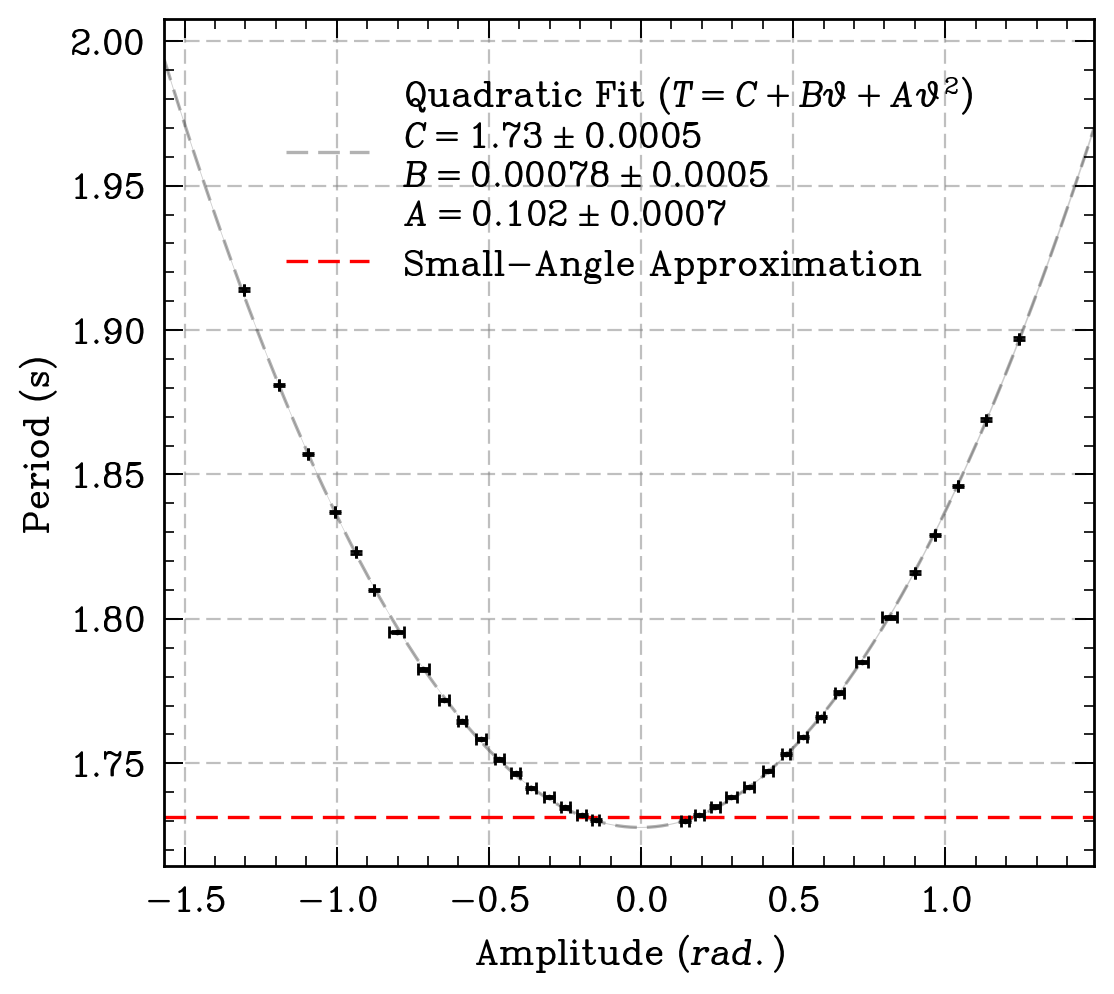
\includegraphics[width=0.9\linewidth]{amp_per_error_of_mean.png}
    \label{fig:amplitude-period}
    \caption{Plot of pendulum period against oscillation amplitude. Datapoint errorbars are calculated using standard deviation ($\epsilon = 1\sigma$). $\theta$ referenced in the legend is the transient amplitude of oscillation.}
\end{figure}

Here we can be confident as the error of $C$ is outside of 2 error margins of 0, meaning it is significant.


\subsection{Damping Factor}

Investigating the damping is a critical part of understanding the pendulum's motion. In a system undergoing quasi-simple harmonic motion (SHM at small timescales), we can define a dimensionless Q factor. The Q-factor can be described in multiple ways, but seems to be most generally defined by equation \ref{eq:qfactor} where $E_\theta$ is the energy at a given $\theta$, wherease $E_{\theta+1}$ is the energy one radian later.

\begin{equation}
    Q=\frac{E_{\theta}}{E_{\theta+1}}
    \label{eq:qfactor}
\end{equation}

Alternatively, it can be found from the exponential damping constant ($Q=\pi\frac{\tau}{T}$). Note that the real pendulum system experiences various damping forces (Couloumb, viscous, and turbulent largely), some of which vary in amplitude as the pendulum's amplitude decreases. This causes the Q-factor to be non-constant across time in our system as visible in Figure \ref{fig:decay}.

\begin{figure}[htb]
    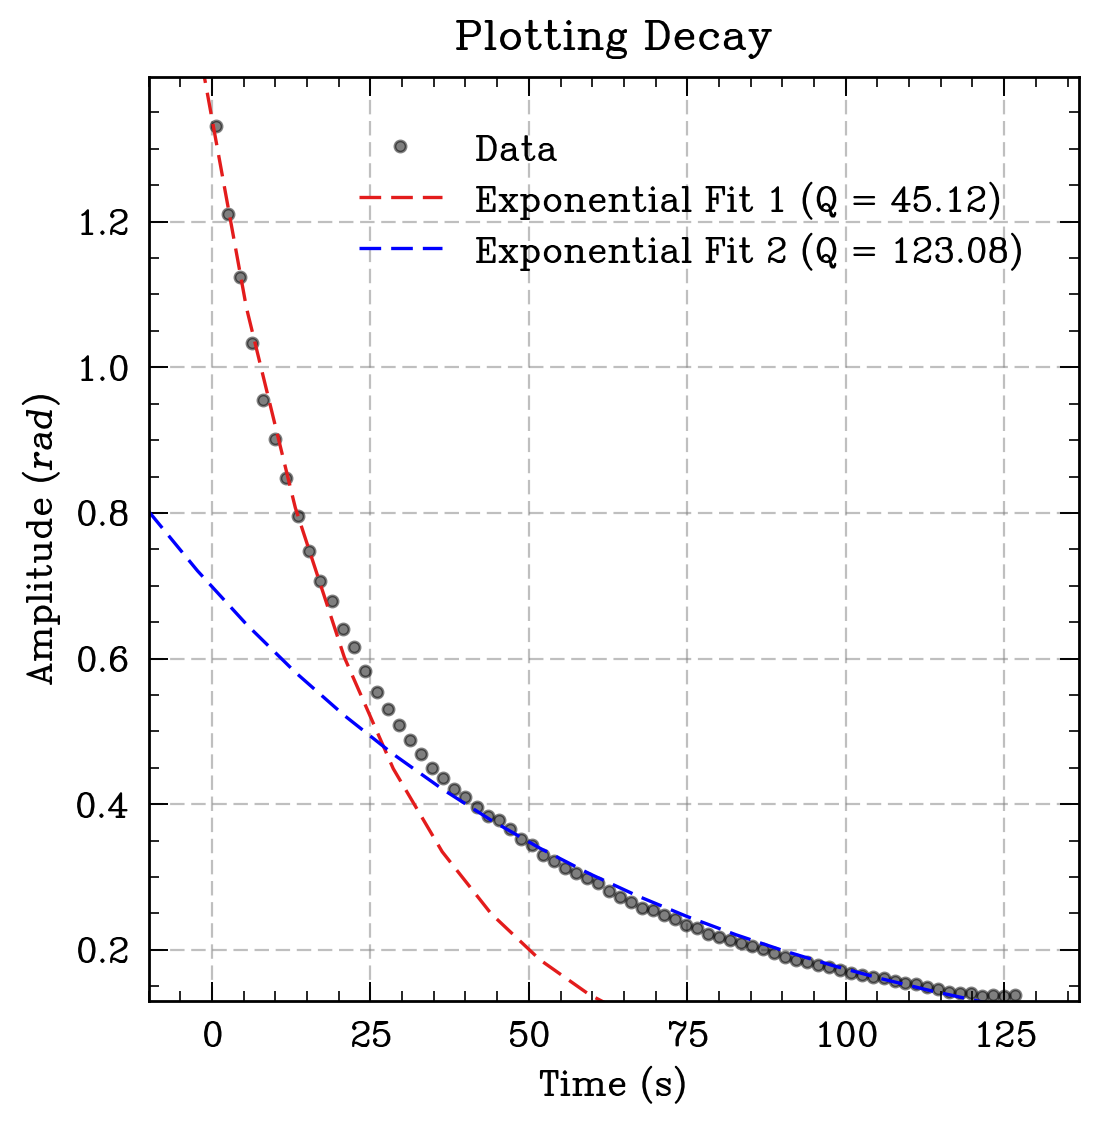
\includegraphics[width=0.8\linewidth]{decay.png}
    \label{fig:decay}
    \caption{Plot of pendulum amplitude against time. Two $\tau$ factors are found for different regions where $t_1\in[0s,25s], t_2\in[75s,125s]$. This shows how a single $\tau$ cannot cover data varying in large rage of amplitudes.}
\end{figure}

Lastly, we can count the Q-factor discretely. By counting the number of full oscillations between $A_0 \Rightarrow [e^{-\pi/15}]A_0$ and multiplying by 15.

\begin{table}[htb]
    \centering
    \caption{Discrete Q-factor calculations based on counted oscillations between $A_0$ and $e^{-\pi/15}A_0$.}
    \vspace{10pt}
    \begin{tabular}{|c|c|c|}
        \hline
        $A_0$ (Starting Amplitude) & Counted Peaks & Q-Factor \\
        \hline
        1.2 radians & 3 & 45 \\
        0.6 radians & 6 & 90 \\
        0.4 radians & 7 & 105 \\
        \hline
    \end{tabular}
    \label{tab:q_factor}
\end{table}

\begin{figure}[htb]
    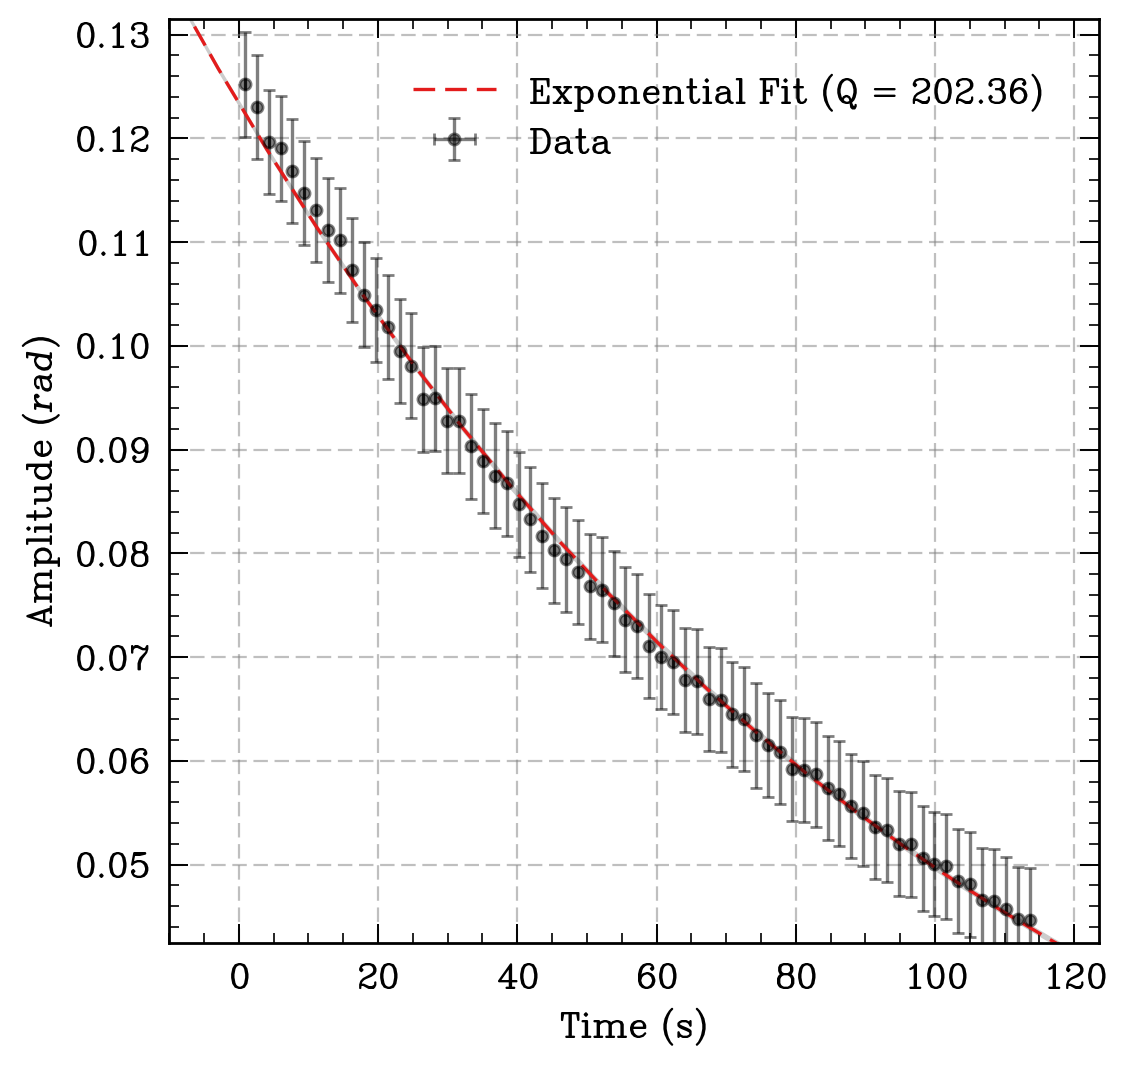
\includegraphics[width=0.8\linewidth]{low_angle_q.png}
    \label{fig:decay_small_angle}
    \caption{Plot of pendulum amplitude against time. Since the range of the amplitudes is smaller in this case, a exponential fits a lot better.}
\end{figure}

\begin{figure}[htb]
    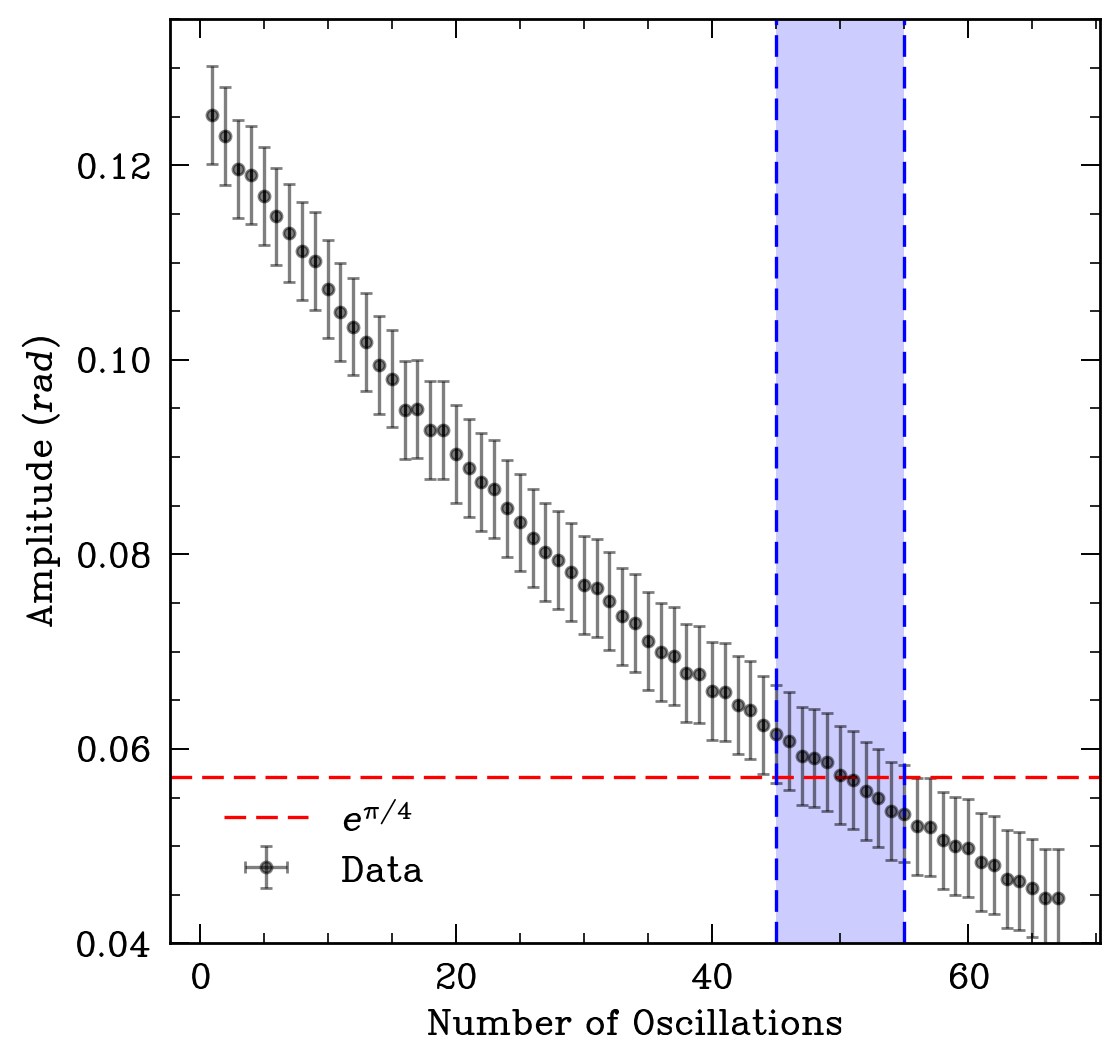
\includegraphics[width=0.8\linewidth]{count_decay.png}
    \label{fig:count_q}
    \caption{Plot of pendulum amplitude against time. Since the range of the amplitudes is smaller in this case, a exponential fits a lot better.}
\end{figure}


\section{Determining Uncertainties}

The uncertainty for the amplitude of the pendulum seen in Figure 6 and 7 are determined through the type-B uncertainty of the amplitude. The width of the pendulum (which it Tracker may not always select the centre of) causes measurement errors. It is calculated as $\epsilon = \frac{w}{2(l)}$ for a 68\% confidence.

\section{Conclusion}
In this report, we investigated the motion of a suspended magnet under the influence of attractive magnets placed on a base.


\onecolumngrid
\newpage

\section{References}

Wilson, Brian, “PHY180 Pendulum Project”, from
\href{https://q.utoronto.ca/courses/411727/files/39071655?module_item_id=7122439}{q.utoronto.ca}, 2025.

\section{Appendix}

\subsection{A. Processing Code}

All of the code I've written for this project is open-sourced on GitHub

\subsection{B. Out-of-plane Oscillations}

In the case that this report investigates, the pendulum has 2 degrees of freedom ($\phi, \theta$). Since the plane that our camera projects is not sensitive to $\phi$, the resultant $\theta$ found is dependent on $\phi$ through $cos(\phi)x_{pendulum} = x_{observed}$.

Thus, tracking the pendulum using a camera, care must be taken to avoid the pendulum going out of plane (in other words, keep $\phi$ at a desirable constant value).

A solution to this is using purely the $y$-tracked values, as these are not dependent on $\phi$ (ignoring parallax, which is not important in our setup).
However, at small angles, these are significantly harder to track due to vanishing derivative $\frac{dcos(\theta)}{d\theta}$ as $\theta \Rightarrow 0$.


\begin{figure}[htb]
    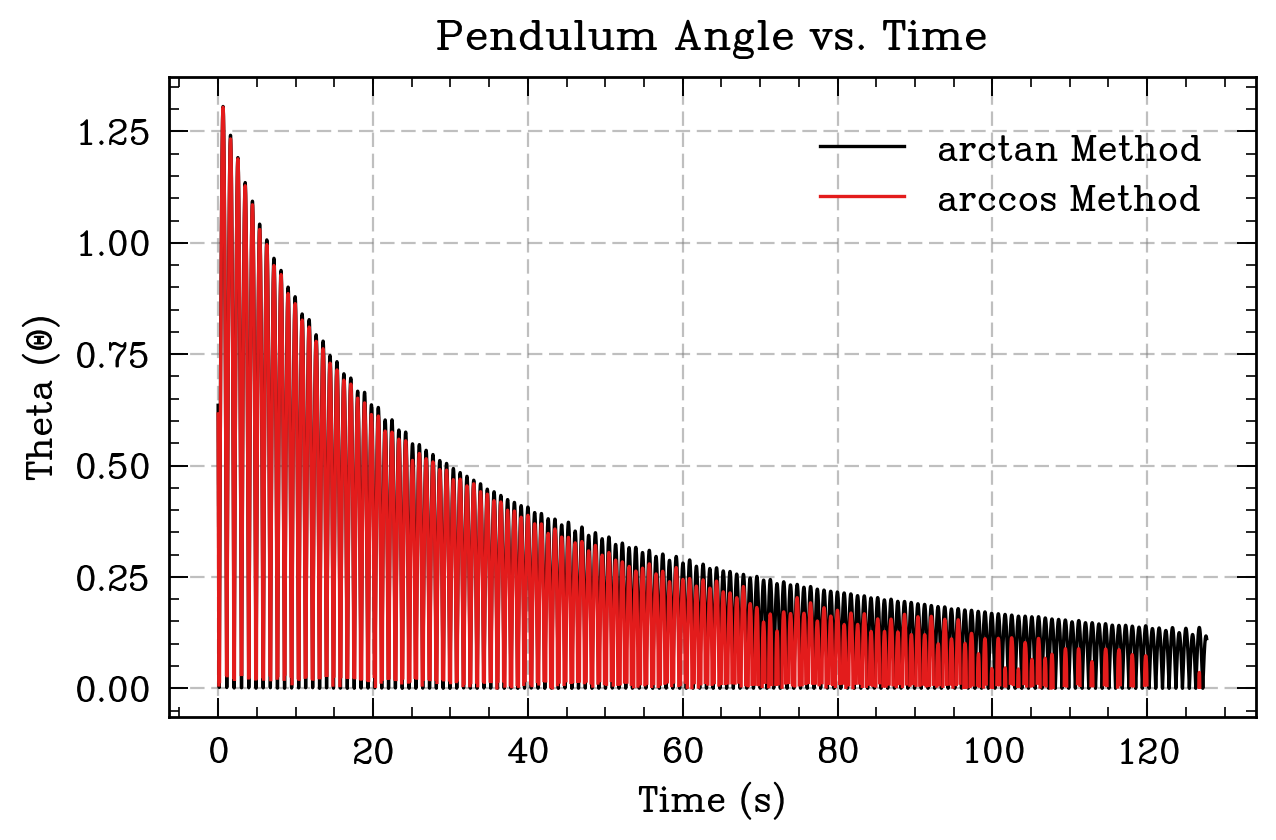
\includegraphics[width=0.5\linewidth]{out-of-plane.png}
    \label{fig:out-of-plane}
    \caption{This graph shows the differences in results between tracking with $\phi$ dependence and without. Note that the reason no negative $\theta$ exists is because that would require us to know $\phi$, something not possible purely from $y$.}
\end{figure}

\subsection{C. Measurement Uncertainty}

\begin{figure}[htb]
    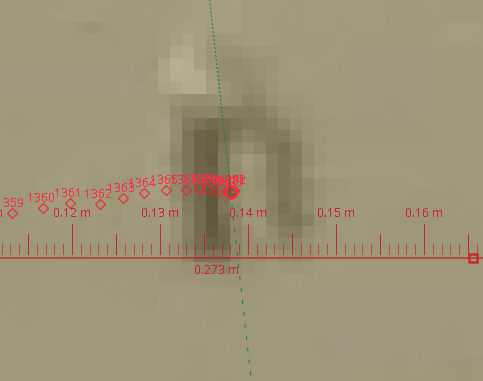
\includegraphics[width=0.3\linewidth]{pendulum-body.png}
    \label{fig:body}
    \caption{This graph shows the differences in results between tracking with $\phi$ dependence and without. Note that the reason no negative $\theta$ exists is because that would require us to know $\phi$, something not possible purely from $y$.}
\end{figure}

\newpage
\subsection{AI Statement}

No form of AI was used in assisting this lab.

\end{document}
